\section{A Review on Early Forest Fire Detection Systems
Using Optical Remote Sensing}

%1
\begin{frame}
    \frametitle{\textit{A Review on Early Forest Fire Detection Systems
Using Optical Remote Sensing ~------~ Overview}}

    There are 3 levels of the smoke and early fire detection system according to
    this review.
    \begin{itemize}
        \item System(platform)
        \item Sensors(types)
        \item Methods(traditional + deep learning based)
    \end{itemize}
    \begin{figure}[H]
        \centering
        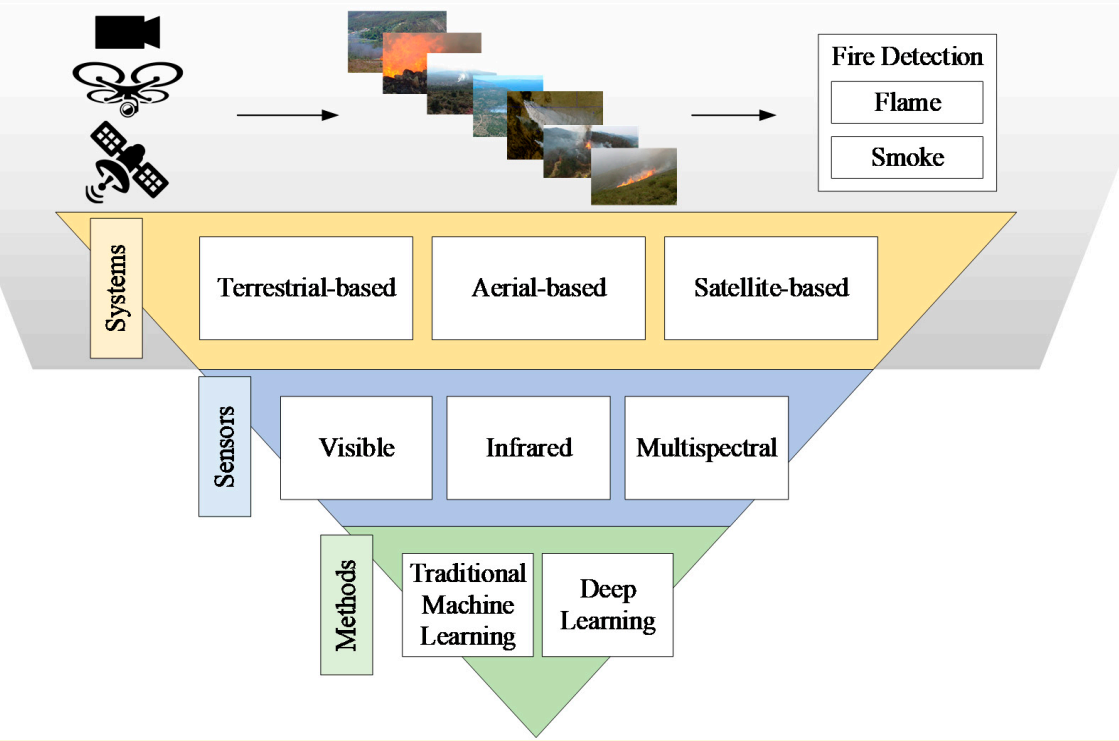
\includegraphics[width=0.6\textwidth]{./imgs/levels}
        \caption{the 3 levels of the detection systems}
    \end{figure}

\end{frame}

%2
\begin{frame}
    \frametitle{\textit{A Review on Early Forest Fire Detection Systems
Using Optical Remote Sensing ~------~ UAV based detection}}

UAVs can provide border and more accurate perception, get through a dangerous
and inaccessible zones.

\begin{columns}[t]
    \column{0.45\textwidth}
    \begin{block}{Traditional}
        \begin{itemize}
            \item noise reducing + color space + threshold = fire segmentation
            \item color space + Kalman filter = smoke detection
            \item color + motion features = fire and smoke segmentation(The
                flame has turbulent features $\rightarrow$ optical flow)
            \item (ROS + SLAM + DJIF550 = navigation) + (color, movement,
                temporal variation of fire intensity) = Simulation implementation
        \end{itemize}
    \end{block}

    \column{0.45\textwidth}
    \begin{block}{Deep learning based}
        \begin{itemize}
            \item Deep convolutional network(15 layers)
            \item Subregion selecting + YOLOv3 backbone + ZenMuse(4k) =
                detection
            \item YOLOv3(on ground station) + UAVs capturing $\rightarrow$ UAV
                flight path planning and replanning.
            \item fog computing + CNN = reducing the false alarm rate.
            \item 360-degree CMOS + DNN + fire dynamic texture = reduce the
                false alarm caused by the sunlight reflection and
                cloud.\footnotemark[1]

        \end{itemize}
    \end{block}

\end{columns}
\footnotetext[1]{The following paper}
\end{frame}
